\chapter{Design and Implementation}
\label{sec:designandimplementation} 

This chapter presents the design and implementation of StoryBook. It first discusses the authors’ journey in dealing with the data in Facebook and the issues inherent in its characteristics. This is followed by the discussion on the event classification algorithm of the system, its issues, initial shortcomings, and improvements. It ends with a discussion of the natural language generation module, which has three submodules: the GenIntro, GenBody, and GenConclusion. The issues encountered during implementation and the solutions applied to address each issue are presented.

%section~~~~~~~~~~~~~~~~~~~~~~~~~~~~~~~~~~~~~~~~~~~~~~~~~~~~~~~~~~~~~~
\section{Processing User-Generated Data}
Facebook was chosen for this research for two reasons, namely: [1] its free-form nature; and [2] the amount of data present in Facebook. From a single Facebook post, plenty of information can already be derived in order to complete events that make up a life story, including, but not limited to: [1] date; [2] time; [3] location; [4] co-participants; [5] a photo, or photos, each of which could have their own separate post filled with their own metadata; and [6] the current activity being done by a person, if they chose to use the \textit{predefined activities} feature.

This does not yet include the actual text content of a single post. From the text post itself, an intelligent machine can be designed to easily determine parts that can be used in natural language generation, such as the subject(s) of the post, the verbs, and the objects they act upon. However, user-generated data such as those from Facebook are inconsistent and noisy (Kinsella et al., 2011). In this section, each of these characteristics are discussed in detail and how the issues inherent in these characteristics are resolved.

\subsection{Brevity of Posts}
\textit{Includes: multi-sentence posts; and very brief posts with implied attributes such as actor, object, or time}

User-generated data in social media is usually brief. Other social networking sites have limitations set in place such that user-generated data is brief on purpose. However, Facebook does not have a set character limit in place, which means that posts on Facebook can be much longer than others. This becomes an issue when a single post contains multiple sentences, each with their own actions and some with different doers. Other posts may be super short, which leads to missing attributes in the text such as the doer, the object, or time.

In dealing with this, long posts with multiple sentences are split into sentences and then parsed per sentence. During preprocessing, Stanford CoreNLP takes care of splitting such post into its constituent sentences, and classification is performed on the individual sentences.

Recall that the story plan is of the form
\begin{center} Verb (doer, receiver of the action, object, date, location) \end{center}

For posts with missing elements in the text needed to fill the story plan, those elements can be found in the metadata instead, or assumed. 
\begin{itemize}
	\item If the \textit{doer} is not mentioned in a given sentence (e.g., ``Had fun today!”), the user who posted it is assumed to be the doer.
	\item If the \textit{receiver} is not mentioned then the poster is assumed to be the receiver.
	\item The \textit{object} can be missing.
	\item The \textit{date} is taken from the post’s metadata.
	\item The \textit{location} can be missing; it is taken from the post’s metadata.
\end{itemize}

\subsection{Informal Nature of Posts}
\textit{Includes: presence of unnecessary characters; presence of foreign characters; emoticons}

Continuing to echo the findings of (Kinsella et al., 2011), posts on social media are more often than not informal, and there is a tendency to resort to hyperlinks or attachments for context. These characteristics were evident in our dataset, wherein it is hard to classify text posts because much of it is humor based around context which a computer cannot know. Also, posts containing foreign characters, emoticons, laughter and hashtags abound. During preprocessing, these were removed as they currently have no relevance to the classification and the generation tasks.

\subsection{Parsing Sentences}
\textit{Includes: POS tagging; multilingualism; parsing sentences with multiple verbs}

Parsing sentences refers to breaking down a post into its different sentences and then breaking down the sentence into its parts and being able to describe their syntactic roles. To do this, POS tagging is done by Stanford CoreNLP. It generates a constituent and dependency representation. From this output, syntactic analysis is performed to extract the necessary event details \cite{Manning14thestanford}.

Given the post ``Going to the mall”. Relevant elements are extracted following these steps:
\begin{itemize}
	\item Extract the verbs that signify the activity described in the post, and the objects or the recipient of the action, which may be another person or object. In this example, the verb is ``going” and the object is the noun phrase describing the destination, ``to the mall”.
	\item Apply lemmatization to transform words to their lemma in order to increase the accuracy of the classifier. In this case, ``going” is lemmatized to ``go”.
\end{itemize}

\begin{figure}[!htb]
	\centering           
	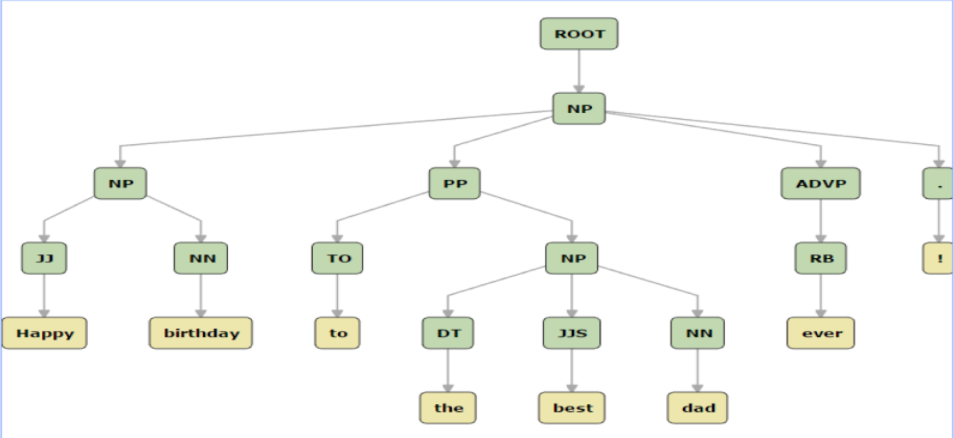
\includegraphics [width=\textwidth] {sf-parsetree.png}    
	\caption{A sample parse tree generated using Stanford CoreNLP}
	\label{fig:sf-parsetree}
\end{figure}

However, the above steps do not work in all cases. Given a sample post -- ``\textit{Happy Birthday to the best dad ever!}”, Stanford CoreNLP generates the parse tree shown in \figref{fig:sf-parsetree}, which contains the tokens, their POS tags and their dependencies. The object is ``\textit{best dad}”; however, the post does not contain any verbs. Posts with no verbs will have to rely on the event classification algorithm to determine its category, in this case, it is a \textit{celebrating} post because of the keyword ``birthday”.

The accuracy of the POS tagging also relies on Stanford CoreNLP, which led to problems because Stanford CoreNLP is not perfect. Depending on the punctuations, for example, a sentence’s POS tagging changes. 

To illustrate, the post, ``Happy friendversary thesismate HAHAHA”, with a tagged person named ``Camille Saavedra,” shows up in the generated story as ``Robee celebrated friendversary thesismate HAHAHA with Camille”. This is because the POS tagger detected ``friendversary thesismate HAHAHA” as the main noun phrase in the post, and so considered it to be the object of the post. POS tagging can also change as a result of multilingual sentences; the use of mixed languages mess up the syntactic structure of the post, making it difficult for the parser to properly perform POS tagging.

After breaking down the sentence and completing the story plan, it is possible to have multiple words in the sentences which leads to the post possibly being classified into multiple types. For example, the sentence, ``Walking while eating gelato,” contains keywords for both \textit{travelling} and eating types of posts.

In the first iterations of the system, the post classification algorithm simply used co-location in order to check which types the post fell under. If it happened to have keywords for different types, the same sentence would appear multiple times in the generated story.

The post classification algorithm was changed: the keywords list was augmented with phrases from WordNet and ConceptNet; a scoring system has been implemented; and multiple post types are no longer possible. This change is further expanded on in Section 5.2, ``Event Classification.”

\subsection{Other Identified Characters}
\textit{Includes: Detecting rumors, contradictory information, sarcasms and humor, onomatopoeia, colloquial language}

Aside from the aforementioned characteristics of social media data, there are plenty of others which do not affect this research, but are relevant to this field. The first is that a lot of information posted online is speculative and wishful. Being able to detect rumors and distinguish them from facts is therefore necessary; however, it is not part of this research. Another characteristic of many posts is humor and/or sarcasm; being able to detect sarcasm and humor is a concern of empathic computing and human-computer interaction, and is not part of this research. Both of these characteristics can affect event detection (because, for example, a sarcastic post can be misconstrued by a computer as fact), and they become more relevant in the future as the topic expands, due to the need to accurately portray users’ lives. Humor and hearsay can be misconstrued by the computer as fact, and therefore, wrong information can be generated.

Other characteristics which are a result of informality on social media include onomatopoeia and colloquial language. Onomatopoeia is the formation of a word from the imitation of a sound associated with it (e.g. ``oink oink”, ``buzz”, or ``haha”). For this research, laughter is removed as part of preprocessing; however, other onomatopoeic sounds are not preprocessed. Colloquial language refers to the use of very informal terms that are not standard; for example, texting in abbreviations (e.g. ``c u l8r”). For the purposes of this research, such language was not taken into consideration.


%section~~~~~~~~~~~~~~~~~~~~~~~~~~~~~~~~~~~~~~~~~~~~~~~~~~~~~~~~~~~~~~
\section{Event Classification}
Although Facebook’s predefined activities feature is designed to enable users to easily classify their individual posts according to content, there are currently no available tools that can support the extraction of relevant elements from posts that use this feature. Furthermore, most Facebook users still prefer the traditional methods when crafting a post, i.e., typing text, and optionally combining photos and videos.

Given this limitation, available tools were used for gathering posts from an individual user's Facebook account, preprocessing the posts, classifying posts according to their event types, and then extracting event details.

\subsection{Keywords (Handcrafted)}
A reference table (shown in \ref{tab:EventClassification}) containing predefined keywords commonly associated with each event category was derived through manual inspection of the dataset. It is important to note that at first, there were 15 types of posts, each with their own co-locating words; later on, it was then trimmed down to four types of posts.
\clearpage
\begin{table}[ph!]   %t means place on top, replace with b if you want to place at the bottom
	\centering
	\caption{Classification of Facebook Posts based on Keywords} \vspace{0.25em}
	\begin{tabular}{|p{1.5in}|p{2in}|} \hline
		\centering Type of Post & Co-Locating Words \\ \hline
		Celebrating & 
			 Birthday \\
			 &  Celebrate \\
		 	&Congratulations \\
			 & Congrats \\
			 & God bless \\		
			 & Bless \\
			 & Wish \\
			 & Happy \\
			 & Merry \\
			 & Party \\
		 \hline
		Traveling & 
			 Go \\ 
			 &  Travel \\ 
			 &  At \\
			 &  Visit \\
			 &  Drive \\
			 &  Road \\
			 &  Place \\
			 &  Far \\
			 &  Run \\
			 &  Walk \\
			 &  Adventure \\
			  & Bucket list \\
		 \hline
		Eating & 
			 Cook \\
			 &  Eat \\
			 &  Dine \\
			 &  Breakfast \\
			 &  Lunch \\ 
			 &  Dinner \\
			 &  Chicken \\
			 &  Burger \\
			 &  Grill \\
			 &  Bake \\ 
			 &  Fry \\
		 \hline
	\end{tabular}
	\label{tab:EventClassification}
\end{table}

For \textit{celebrating} events, words which usually indicate special events such as \textit{birthdays} and \textit{Christmas} are used. For posts on \textit{travelling}, synonyms as well as methods of traveling are used. For \textit{eating}, aside from synonyms, the meals of the day are also used as indicators.

Since the dataset derived from manual inspection is by no means exhaustive of all Facebook user accounts, the list of keywords is not complete, and needed to be expanded to improve the classification process. 

\subsection{Keywords from Existing Resources (ConceptNet and WordNet)}
In order to address the issue of lack of keywords, the combination of the outputs of the two lexical resources, WordNet and ConceptNet, were used to populate the keywords list to be used later for event classification (as shown in \ref{tab:EventClassificationWordNet} and \ref{tab:EventClassificationConceptNet}). 

Initially, the plan was only to use WordNet only by extracting related concepts through its related senses. However, the lexical knowledge contained in WordNet was found to be insufficient for our purpose, as many terms (specifically physical objects) do not exist in it. To increase the coverage, ConceptNet’s lexical and semantic knowledge was utilized to derive related contexts in which the words \textit{celebrating}, \textit{travelling}, \textit{eating}, and \textit{drinking} are found. Specifically, all semantic relations except antonym relation were used to derive the concepts. ConceptNet also contained a very minimal amount of Filipino words; these were also extracted to handle posts that contain Filipino words. An example Filipino word, \textit{paglalakbay}, is shown in \ref{tab:EventClassificationConceptNet} as one of the keywords for the \textit{travelling} post.
\clearpage
\begin{table}[ph!]   %t means place on top, replace with b if you want to place at the bottom
	\centering
	\caption{Classification of Facebook Posts Based on Words Identified Through WordNet} \vspace{0.25em}
	\begin{tabular}{|p{1.5in}|p{2in}|} \hline
		\centering Type of Post & Co-Locating Words \\ \hline
		Celebrating 
			& Celebrate \\
			& Observe\\
			& Fete\\
			& Lionize
		\\ \hline
		Eating 
			& Eat\\
			& Feed\\
			& Depletion\\
			& Consume 
		 \\ \hline
		Drinking 
			& Booze\\
			& Salutation\\
			& Pledge\\
			& Salute\\
			& Toast
		 \\ \hline
		Traveling
			& Movement\\
			& Traveler\\
			& Locomotion\\
			& Journey\\
			& Trip\\\hline
	\end{tabular}
	\label{tab:EventClassificationWordNet}
\end{table}
\clearpage
\begin{table}[ph!]   %t means place on top, replace with b if you want to place at the bottom
	\centering
	\caption{Classification of Facebook Posts Based on Words Identified Through ConceptNet} \vspace{0.25em}
	\begin{tabular}{|p{1.5in}|p{2in}|} \hline
		\centering Type of Post & Co-Locating Words \\ \hline
		Celebrating 
			& Victory \\ 
			& Christmas \\ 
			& Firework \\ 
			& Birthday \\ 
			& Toast \\\hline
		Eating  
			& Chew \\ 
			& Swallow \\ 
			& Food \\ 
			& Cook \\ 
			& Plate \\ 
			& Kain \\\hline

		Drinking 
			& Thirsty \\ 
			& Liquid \\
			& Bottle \\ 
			& Beer \\ 
			& Lemonade \\ 
			& Inumin \\\hline
		Traveling 
			& Passport \\ 
			& Fun \\ 
			& Explore \\ 
			& Pack \\ 
			& Adventure \\ 
			& Paglalakbay  \\\hline
	\end{tabular}
	\label{tab:EventClassificationConceptNet}
\end{table}

Currently, the system has 1,697 co-locating words across all event types. Table \ref{tab:Co-locatingWords} shows a breakdown of the co-locating words.
\begin{table}[ph!]   %t means place on top, replace with b if you want to place at the bottom
	\centering
	\caption{Distribution of the co-locating words per event type and source} \vspace{0.25em}
	\begin{tabular}{|p{1in}|c|c|c|} \hline
		\centering Event Types & from WordNet & from ConceptNet & TOTAL \\ \hline
		Celebrating & 9 & 350 & 359 \\ \hline
		Eating & 17 & 400 & 417 \\ \hline
		Drinking & 24 & 492 & 516 \\ \hline
		Traveling & 16 & 389 & 405 \\ \hline
		TOTAL & 66 & 1631 & 1697 \\ \hline
	\end{tabular}
	\label{tab:Co-locatingWords}
\end{table}

\subsection{Scoring System}
As stated in 5.1.3, posts are classified by their relevant keywords. This is done by first breaking down the post into its individual sentences and getting the part-of-speech tags of each token, which is handled by Stanford CoreNLP. Afterwards, the verbs are lemmatized, and all relevant tokens in the sentence are cross-referenced with the table of classification stated in 5.2.1.

Because a single sentence can contain multiple verbs or words signifying events, the first iteration of the automated classifier classified this into multiple event categories. For example, the sentence, ``\textit{Walking around the streets of Rome while eating delicious gelato,}” was classified as an eating event and a travelling event. 

To avoid redundancy and the loss of context in downstream tasks, the classification algorithm has been revised to use a scoring system, and the sentence is assigned the category with the highest score. If multiple event categories bear the same score, a bias scheme based on the hierarchy of \textit{celebrating} =$>$ \textit{eating} =$>$ \textit{drinking} =$>$ \textit{travelling} will be followed. A threshold value of 2 was also set to minimize the occurrence of misclassification. 

Consider the sentence, ``\textit{I’d love to take a walk on the park someday.}” The presence of the word walk in the list of keywords led the no-score classifier to consider this sentence as a travelling event, when it should not have been the case. In the score-based classifier, only sentences such as ``\textit{I’m going on an adventure to check off one from the bucket list}”, which has a score of 3 because of the words ``\textit{going}”, ``\textit{adventure}”, and ``\textit{bucket list}	” and thus, was categorized as a \textit{travelling} event.

%section~~~~~~~~~~~~~~~~~~~~~~~~~~~~~~~~~~~~~~~~~~~~~~~~~~~~~~~~~~~~~~
\section{Life Story Generation}
The text generation module is responsible for generating the appropriate story segments that make up the entire life story generated by the system. There are three components of the text generation module, namely the GenIntro, GenBody, and GenConclusion. GenIntro is the module applied to the data determined to be “facts” or direct knowledge, such as family and work information; GenBody is applied to generate the body of the life story from the data processed in the Data Processing module; and GenConclusion is the module applied to the data determined to be “facts” or direct knowledge.

Following the NLG pipeline of Reiter \& Dale (1997; 2000), story generation usually proceeds in three main steps, namely content determination, discourse planning, and surface realization. Initially, the system used a template-based generation algorithm, but later switched to a grammar-based (or script-based; the two terms are interchangeable in the context of our research) algorithm. A thorough discussion of the rationale behind the switch is explained in Section 5.3.6 Switching to Grammar-Based Generation.

\subsection{Template-Based Generation}
Following the NLG pipeline mentioned earlier, content determination for GenIntro and the GenConclusion involve deriving data supplied by the user themselves. The system initially used templates and was therefore \textit{template-based}. For example, when generating the introduction, the system follows a fixed template of:
\begin{itemize}
	\item $<$NAME$>$ $<$\textit{birth circumstance}$>$ $<$\textit{current education}$>$ $<$\textit{location}$>$ $<$\textit{family}$>$
\end{itemize}

Then, each of these has their own sub-templates. For instance, $<$\textit{birth circumstance}$>$ can choose from the following templates:
\begin{itemize}
	\item $<$\textit{intro\_birth\_circumstance}$>$
	\item Is a $<$AGE$>$-year old $<$GENDER$>$ who
\end{itemize}

Then, the $<$\textit{intro\_birth\_circumstance}$>$ can still be broken down to other sub-templates such as:
\begin{itemize}
	\item , born on $<$BIRTHDAY$>$,
	\item was born on $<$BIRTHDAY$>$
\end{itemize}

And then, upon choosing the templates at random, the system would then fill in the blanks with the data stored in the \textit{direct knowledge} table as follows:

\begin{center} Robee, is a 21-year old female who has yet to get her college diploma from De La Salle University. \end{center}


The system would then chain templates like these together in order to create the introductory and conclusion paragraphs. Following the NLG pipeline mentioned earlier, this would be discourse planning, but very minimal discourse planning is performed in a template-based approach due to how simple it is.  Each time, it would have to choose a sentence at random. This poses a problem: the templates are manually created by a person, and so if a new sentence type were to be implemented, such as about a person’s phone number, a template would have to be created, which includes all possible varieties of sentences that can be formed which talk about the phone number. Also, note that since templates are not flexible, it introduces problem for surface realization: there are usually grammar problems encountered such as the use of the correct pronoun or the correct preposition. These would then have to be worked around by the system, which means more work had to be done.

Therefore, a way to dynamically generate sentences using NLG is needed for extensibility and scalability. Works such as (\cite{chen2008natural}; \cite{sleimi2016generating}) have shown the power of using RDF data to construct descriptive sentences dynamically. This approach was adapted, which enabled support for graph-based, or grammar-based, text generation, using scripts instead of templates. 

This meant that the story planning and the surface realization parts are changed, since the content determination stays the same.

\subsection{Scripts}
The story generator uses RDF data to construct sentences, with the help of SimpleNLG. RDF data consists of (\textit{subject property object}) triples such as (\textit{Robee, nationality, Taiwanese}). As illustrated in \figref{fig:rdf}, RDF data can be represented by a graph in which edges are labelled with properties and vertices with subject and object resources.

\begin{figure}[!htb]
	\centering           
	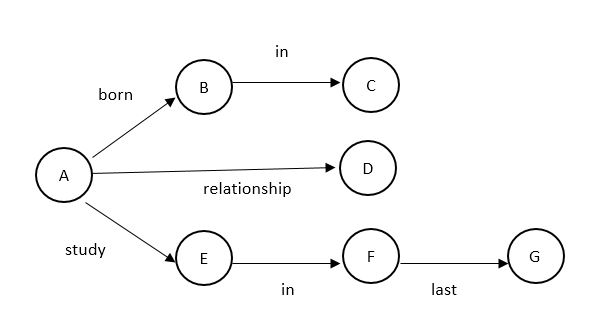
\includegraphics  [width=4.5in,height=4.2in,keepaspectratio] {graph-rdf.jpg}    
	\caption{An example of a graph representation of RDF data. (A, birthPlace, F) is connected to (F, country, H), for example. }
	\label{fig:rdf}
\end{figure}

Each vertex in the graph is an object (not to be confused with \textit{direct object}), and for the purposes of story generation, each object is described in a sentence (turning it into an assertion or a message). Aside from the name of the object, assertions can be a combination of the following.

For the introduction, the assertions are:
\begin{itemize}
	\item person (lastName, firstName, middleName)
	\item gender(obj)
	\item livingIn(obj)
	\item family(relationship, names$<$$>$)
	\item roleFam(obj)
	\item occupation(obj)
	\item birth(date, place)
	\item education(institution, type, yeargrad, course)
	\item work(institution, startDate, endDate, location)
\end{itemize}

And for the conclusion:
\begin{itemize}
	\item person (\textit{lastName, firstName, middleName})
	\item eventsGoing(\textit{name, location})
	\item eventInterested(\textit{name, location})
	\item likes(\textit{category, page$<$$>$})
\end{itemize}
These assertions are then filled with information from the user data, such that, for example,

\begin{center} person (lastName, firstName, middleName) \end{center}

becomes

\begin{center} person (Hade, Alden Luc, Rosqueta) \end{center}

A set of story grammar rules were used to form English sentences.

The grammar rules used for the introduction are shown in \ref{tab:GrammarRules}; for the body, Table 2369; and the rules used for the conclusion are shown in \ref{tab:GrammarRules-Conclusion}. (\ref{tab:GrammarRules} here as an example; the grammar rules for the conclusion and body are in their respective sections later on.)

\begin{table}[ph!]   %t means place on top, replace with b if you want to place at the bottom
	\centering
	\caption{Grammar Rules Used for the Introductory Paragraphs} \vspace{0.25em}
	\begin{tabular}{|p{2in}|p{2.5in}|} \hline
		$<$INTRODUCTION$>$ &$<$SENTENCE$>$+ \\ \hline
		$<$SENTENCE$>$ & $<$subject$>$ $<$PREDICATE$>$ \\ \hline
		$<$PREDICATE$>$ & $<$verb$>$ $<$OBJECT$>$ \\ \hline
		$<$OBJECT$>$ & $<$noun$>$ [$<$preposition phrase$>$*] $|$$|$ \newline
		$<$article$>$ $<$noun$>$ [$<$preposition phrase$>$*] $|$$|$\newline
		$<$preposition phrase$>$ \\ \hline
	\end{tabular}
	\label{tab:GrammarRules}
\end{table}
The system reads the grammar file using the bottom up approach, where it will start with filling the grammar rules at the bottom with data, before working its way up. Grammar rules that have not been filled up will be removed, while grammar rules that have been filled will be used to generate the assertion. The system then loops through the list of assertions for the introduction and conclusion, fills them with data, generates the sentences with the help of the grammar rules, and puts the sentences together, in order to generate the paragraphs for the introduction and conclusion respectively. 

An example for the introduction would be that the following assertions

\begin{center} person (lastName, firstName, middleName) \end{center}
\begin{center} gender(gender) \end{center}
\begin{center} livingIn(location) \end{center}

with the help of data from Facebook would become

\begin{center} person (``Te'', ``Robee Khyra Mae'', ``'') \end{center}
\begin{center} gender(``Female'') \end{center}
\begin{center} livingIn(``Manila, Philippines'') \end{center}

and would generate the following RDF triples (note that the surface form of the verbs are defined as part of the RDF triples):

\begin{center} (``Robee Khyra Mae Te'' ``is'' ``female'') \end{center}
\begin{center} (``Robee Khyra Mae Te'' ``lives in'' ``Manila, Philippines'') \end{center}

Each of these RDF would then become a sentence of the form

\begin{center} $<$sentence$>$	-$>$	$<$subject$>$ $<$predicate$>$ \end{center}

where

\begin{center} $<$predicate$>$	-$>$	$<$verb$>$ $<$object$>$ \end{center}

Therefore, the generated sentences would become

\begin{center} Robee Khyra Mae Te is female. \end{center}
\begin{center} Robee Khyra Mae lives in Manila, Philippines. \end{center}

Putting the sentences next to each other would result in a paragraph. 

\subsection{Generating the Introduction}
The introduction paragraphs are meant to present the Facebook user to the reader, to provide a background of the subject as if in a real biography. The very first test of the NLG was done simply to check whether the data is being used correctly, and how well the templates would look when put together into a paragraph. The templates were simply filled up and concatenated with each other. Since each template was not a complete sentence by itself but rather a clause, the output paragraph was not separated into sentences. Also, templates which were not filled with data would glaringly have missing information. An example of this is shown below.

\begin{center} Robee Khyra Te was born \underline{\textbf{on 05/25/1996 got her high school diploma}} from Chiang Kai Shek College \underline{\textbf{in 2013 graduated college}}  in De La Salle University \underline{\textbf{last 0 worked from}} 2013-09-01 to 2014-04-30 at University Student Government, \underline{\textbf{DLSU is from $<$hometown$>$}} she is the daughter of Ian Quintin and Katherine Ann Te.
 \end{center}

For the first true iteration of GenIntro, these templates were put together into sentences with the help of SimpleNLG. However, it still could not account for missing information:

\begin{center} Robee Khyra Te was born on 05/25/1996. \underline{\textbf{She got his high school}} diploma from Chiang Kai Shek College in 2013. \underline{\textbf{She got his college diploma from De La Salle University on $<$grad\_year$>$.}} She worked from \underline{\textbf{2013-09-01 to 2014-04-30}} at University Student Government, DLSU. She hailed from Manila, Philippines, and is now living in Manila, Philippines. \underline{\textbf{She she}} is the daughter of Ian Quintin and Katherine Ann Te.
 \end{center}

Worth noting is that the template in the database, since it was created by a human, assumed a lot of things about what the computer can do by itself (such as the simple issue of separating the paragraph into sentences, or determining the user’s gender). 

For the next iterations, the missing information were accounted for. If a template cannot be filled completely, clauses related to the missing information (such as the dependent clause ``from $<$hometown$>$”) are removed. However, the text was still not completely readable. Dates were listed as they are in the database rather than written like natural language. The introduction text also still did not know if a student has graduated already or is still studying, for example. Also, the gender of the subject was not yet determined, so there are contradicting pronouns in the paragraph.

And so the generation was further improved. The gender of the user was eventually  determined correctly; dates were made readable; and the system now took into account the years of education or work in order to determine whether they happened in the past or not, and then explain them in a way that makes sense. Another problem was redundant data: if the current city and hometown are the same, the same town appeared twice, perhaps even in the same sentence.

The last iteration before switching to grammar-based story generation produced an introduction which provides a concise, coherent, and grammatically-correct description of basic information about the subject’s life.

\begin{center} Robee Khyra Te, born on \underline{\textbf{May 25, 1996}}, got her \underline{\textbf{high school diploma}} from Chiang Kai Shek College \underline{\textbf{last 2013}}. She \underline{\textbf{has yet to get}} her college diploma from De La Salle University. She worked from \underline{\textbf{September 01, 2013 to April 30, 2014}} at University Student Government, DLSU. \underline{\textbf{She is from Manila, Philippines.}} She is the daughter of Ian Quintin and Katherine Ann Te. \end{center}

The grammar rules for the grammar-based story generation of the body are shown in \ref{tab:GrammarRules}.

\subsection{Generating the Conclusion}
The conclusion is meant to summarize what was said about the user in the body of the life story by stating their likes. These likes are supported by giving examples of related Facebook pages that the user has Liked. But the conclusion also provides support to these likes by providing examples of events attended by the person.

The initial output did not have any limit as to how long it would be, and so all of the user’s likes and the events they attended were slammed into the paragraph. This was quickly corrected by limiting the conclusion paragraph(s) to three Liked pages per type.

\begin{center} Robee Khyra Te likes \underline{\textbf{Community}} such as Technology Impact Summit 2017, RVR COB Week 2017, \underline{\textbf{A}}nnyeong Oppa. \newline
	\underline{\textbf{Robee Khyra Te likes Artist}} such as Calleftgraphy, Park Shin Hye-PSH ë°?ì? í??\underline{\textbf{, S}}ong Hye Kyo. \newline
	\underline{\textbf{Robee Khyra Te likes TV Show}} such as Cinderella and Four Knights, Moonlight Drawn by Clouds - Korean Drama, \underline{\textbf{D}}escendants of the Sun. \end{center}

The problems dealt with in the improvement of the conclusion paragraph(s) were all related to grammar and punctuation and capitalization errors. However, first, there was the need to teach the generator to use pronouns, because saying the full name in each sentence is redundant. Some of the simple sentences to form longer sentences were then combined, once the system was taught to use pronouns:

\begin{center} Robee Khyra Te \underline{\textbf{likes Communities}} such as Technology Impact Summit 2017, RVR COB Week 2017 \underline{\textbf{, A}}nnyeong Oppa \underline{\textbf{., Artists}} such as Calleftgraphy, Park Shin Hye-PSH ë°?ì? í??\underline{\textbf{, S}}ong Hye Kyo\underline{\textbf{., TV Shows}} such as Cinderella and Four Knights, Moonlight Drawn by Clouds - Korean Drama\underline{\textbf{, D}}escendants of the Sun. \end{center}

Finally, the events attended by the user were plugged into the conclusion.
\begin{center} Robee Khyra Te likes communities such as Technology Impact Summit 2017, RVR COB Week 2017, Annyeong Oppa, artists  such as Calleftgraphy, Park Shin Hye-PSH ë°?ì? í??, Song Hye Kyo, TV shows  such as Cinderella and Four Knights, Moonlight Drawn by Clouds - Korean Drama, Descendants of the Sun. \newline 
Robee Khyra Te attended Cybersecurity and International Relations, Publication Writing Workshop, LSCS Christmas Party! at The Manila Residences Tower II in Manila, CCS Month 2016: Festivo at Henry Sy Bldg, De La Salle University - Manila and Technology Summit 2016 Forum at De La Salle University in Manila. 
 \end{center}
 The grammar rules for the grammar-based generation approach for the conclusion paragraphs are shown in \ref{tab:GrammarRules-Conclusion}.
 \clearpage
\begin{table}[ph!]   %t means place on top, replace with b if you want to place at the bottom
	\centering
	\caption{Grammar Rules Used for the Conclusion Paragraphs} \vspace{0.25em}
	\begin{tabular}{|p{2in}|p{2.5in}|} \hline
		$<$CONCLUSION$>$ & $<$SENTENCE$>$+ \\ \hline
		$<$SENTENCE$>$ & $<$subject$>$ $<$verb$>$ $<$PHRASES$>$ \\ \hline
		$<$PHRASES$>$ & $<$SIMPLE\_PHRASE$>$ $|$$|$ \newline $<$COMPLEX\_PHRASE$>$ \\ \hline
		$<$SIMPLE\_PHRASE$>$ & $<$NOUN\_PHRASE$>$+ \\ \hline
		$<$NOUN\_PHRASE$>$ & $<$noun$>$ $<$LIST$>$ \\ \hline
		$<$LIST$>$ & ``such as” ($<$noun$>$ [$<$prepositional phrase$>$*])+ \\ \hline
		$<$COMPLEX\_PHRASE$>$ & $<$GERUND\_PHRASE$>$ $<$INFINITIVE\_PHRASE$>$ $<$LIST$>$ \\ \hline
		$<$GERUND\_PHRASE$>$ & in $<$verb$>$ \\ \hline
		$<$INFINITIVE\_PHRASE$>$ & to $<$noun$>$ \\ \hline
	\end{tabular}
	\label{tab:GrammarRules-Conclusion}
\end{table}

The outputs for grammar-based story generation for both introduction and conclusion are similar, with the most significant changes happening under the hood rather than on the surface (or the generated story, in this case).

\subsection{Generating the Body}
The body is meant to show events regarding \textit{celebrating, eating, drinking,} and \textit{travelling}, with the observation that these posts are most explicitly stated by Facebook users. The bulk of the work for the story generator is in producing the text for the body of the life story. Following the NLG pipeline mentioned earlier, content determination involves utilizing the events that were derived from processing and classifying the posts. Story planning is then responsible for organizing and sequencing the events into a coherent story plan, which is comprised of sequences of events of the form

\begin{center} Verb (doer, receiver of the action, object, date, location) \end{center}

In generating the story plan, the planner takes into consideration the temporal and the topical relations of events. Topical relations are used to generate paragraphs; one topic (or event category) equates to one paragraph. Within each paragraph, events are ordered based on their temporal relations, which are determined from the timestamps attached to each post and linked to the corresponding events.

Surface realization converts each verb entry in the story plan into a sentence to express the date(s) of occurrence, as well as the people and places involved in each event. The task involves defining the input specifications for each sentence to be generated. This includes setting the user and other people tagged as the actor or doer of the action, the particular action, the object, and the tense of the verb.

\begin{table}[ph!]   
	\centering
	\caption{Sample Facebook posts classified as \textit{celebrating} posts, along with their metadata} \vspace{0.25em}
	\begin{tabular}  {|p{2in}|p{1.5in}|p{1.5in}|}  \hline
    \multicolumn{1}{|c|}{Original Post} & \multicolumn{2}{c|}{Metadata}\\ \hline
	Happy 18th Angie! &  date created & 10/03/14 \\ \hline
	
	{Happy anniversary Jamie HAHA} &  {date created} &{02/07/17} \\\cline{2-1}
	& {user tagged} & {Jamie} \\\hline
	
	{Happy friendversary thesismate!} &  {date created} & {02/14/17} \\\cline{2-1}
	&  {user tagged} &{Cam} \\\hline
	
	{Party party!} &  {date created} & {08/16/16} \\\cline{2-2}
	&  {user tagged} & {Shane} \\\cline{2-2}
	&  {location} & {Manila, Philippines} \\\hline
	
	\end{tabular}
	\label{tab:GrammarRules-celeb}
\end{table}

Consider the Facebook posts including the extracted metadata shown in Table \ref{tab:GrammarRules-celeb}, all classified as celebrating. The corresponding story plan is

\begin{center} celebrating(Mae, null, Angie, 10/03/14, null) \newline
	celebrating(Mae, null, Jamie, 02/07/17, null) \newline
	celebrating(Mae, null, thesismate, 02/14/17, null) \newline
	celebrating(Mae, null, null, 08/16/16, null) \end{center}

and the resulting story text is

\begin{center} On October 03, 2014, Mae celebrated Angie. On February 14, 2017, Mae celebrated thesismate with Cam. On August 16, 2016, Mae celebrated with Shane in Manila, Philippines. On February 07, 2017, Mae celebrated Jamie HAHA with Jamie. \end{center}

This is actually the one of the earlier iterations of the body of the story. In the early iterations of \textit{GenBody}, each event leads to one sentence of the form ``\textit{On $<$date$>$, $<$actor$>$ celebrated $<$activity$>$ with $<$friend$>$.}” Before that, the dates were not even mentioned at all, and the activities identified were almost always wrong:

\begin{center} Robee Khyra \underline{\textbf{celebrated Copyright Infringement Intended.}} Robee Khyra celebrated \underline{\textbf{Angeline.}} Robee Khyra celebrated \underline{\textbf{Janine Tan HAHA.}} Robee Khyra celebrated \underline{\textbf{thesismate.}} \end{center}

One solution to improve the coherency and reduce the redundancy in the generated text is to take advantage of the temporal relations among events by sorting them from most recent to oldest according to their timestamp. This task is handled by the story planner. The surface realizer then applies aggregation to group related events together, i.e., those with closer temporal relations or those with the same people involved. Closer temporal relations mean either the same date, the same month or the same year.

Mae \underline{\textbf{has celebrated most with}} Shane, Jamie and Cam. They celebrate together. A year ago, she celebrated with Shane mid-July. A few months ago, she celebrated friendversary with Cam. A few months earlier, she celebrated \underline{\textbf{anniversary jamie}} with Jamie.

The problems encountered with this approach stem mostly from difficulty in parsing posts that are mostly informal in nature. Some posts are parsed incorrectly, leading to the wrong activity being articulated. For example, in the last sentence above, the identified activity from the post is “anniversary jamie”.

Similar to GenIntro and GenConclusion, the GenBody has been modified to accept data of RDF triples, and thus the generation also becomes grammar-based. The grammar rules for this are shown in Table \ref{tab:GrammarRules-bodypar}.

\clearpage
\begin{table}[ph!]   
	\centering
	\caption{Grammar Rules Used for the Body Paragraphs} \vspace{0.25em}
	\begin{tabular}{|p{2.4in}|p{3in}|} \hline
		{$<$BODY$>$}  & {$<$SENTENCE$>$+} \\ \hline
		$<$SENTENCE$>$ & $<$SENTENCE\_SPECIFIC$>$ $|$$|$ $<$SENTENCE\_SUMMARIZED$>$ \\ \hline
		$<$SENTENCE\_SPECIFIC$>$ & $<$time$>$ $<$subject$>$ $<$PREDICATE\_SPECIFIC$>$\\ \hline
		$<$PREDICATE\_SPECIFIC$>$ & $<$verb$>$ $<$OBJECT\_SPECIFIC$>$ \\ \hline
		$<$OBJECT\_SPECIFIC$>$ & "to" $<$noun$>$ $<$LOCATION\_SPECIFIC$>$ $<$PEOPLE\_TAGGED$>$ \\ \hline
		$<$LOCATION$>$ & "at" $<$noun$>$ \\ \hline
		$<$PEOPLE\_TAGGED$>$ & "with" $<$noun$>$+ \\ \hline
		$<$SENTENCE\_SUMMARIZED$>$ & $<$subject$>$ $<$PREDICATE\_SUMMARIZED$>$\\ \hline
		$<$PREDICATE\_SUMMARIZED$>$ & $<$verb$>$ $<$OBJECT\_SUMMARIZED$>$ \\ \hline
		$<$OBJECT\_SUMMARIZED$>$ & $<$noun$>$ $<$PREP\_PHRASE$>$ \\ \hline
		$<$PREP\_PHRASE$>$ & $<$PLACE\_PHRASE$>$ $<$CITY\_PHRASE$>$ $|$$|$ \newline $<$LIST$>$ $|$$|$ \newline $<$PEOPLE\_TAGGED$>$ \\ \hline
		$<$PLACE\_PHRASE$>$ & "to" $<$noun$>$+ $|$$|$ \newline "at" $<$noun$>$+ \\ \hline
		$<$CITY\_PHRASE$>$ & "in" $<$noun$>$ \\ \hline
		$<$LIST$>$ & ``such as” $<$noun$>$+ \\ \hline
	\end{tabular}
	\label{tab:GrammarRules-bodypar}
\end{table}

Worth noting is that for GenBody, two types of sentences can be formed. These can either be sentences talking about a specific post, or a generalization or summary of multiple posts. An example of a specific sentence would be, “He went to the mall with Janica at Glorietta,” while an example of a summary sentence would be, ``He celebrated the most with Janica, Robee, Alden and Camille.”

\subsection{Switching to Grammar-Based Generation}
The structure used for the paragraphs of the life stories generated in this research, as well as the switch from template-based generation to grammar-based generation (in the form of scripts), is in part based on the work of \cite{Tuffield06ontologicalapproaches}.

When modeling a story, it is important to take note of the structure of \textit{fabula} items; in the case of the system, the fabula refers to story elements such as characters, objects, and events. The structure is enforced by grammar rules-- and these grammar rules are often enforced by templates.

However, as discovered over the course of this research, templates are rigid and have to first be defined by developers every time a pattern needs to be created. This limits the flexibility and scalability of the system. For example, if there exists a template for a sentence which introduces simply the user’s name, the developer would have to define each different variation that can be produced by following this template. For example:

\begin{center}
\begin{itemize}
	\item $<$name\_nickname$>$ $<$optional\_clause$>$ $<$current\_job\_or\_education$>$
	\item $<$name\_nickname$>$ $<$optional\_clause$>$ $<$birth\_circumstance$>$
	(and then each of those elements except for \textit{name\_nickname} would have to be created manually as well, since they are not terminals; similar to the example in Section 5.3.1 Template-Based Generation)
\end{itemize}
\end{center}

If an end-user wanted more variations, the developers would have to manually define new variations. Worse still, if an end-user wanted to define new sentence types not accounted for, the developers would have to manually define each sentence type (e.g. introducing a person’s pet, or birthday, or relationship status), and manually create each \textit{variation} within each sentence type. This results in additional overhead which could have been solved by using grammar rules instead and allowing tools such as SimpleNLG to focus on surface realization.

This is why the system switched to grammar-based story generation instead: easier definitions and an aim for greater flexibility and scalability. In this case, it is now possible to generate varying sentences for the paragraphs without having to manually define new templates: the focus then goes to the grammar and the script. As stated by (Tuffield, 2006), ``ontologies built around existing narrative theory offer a powerful way to tackle this problem at a more pragmatic level, without encumbering end users with additional overheads of conceptualising explicit semantics.”

